\documentclass[defaultpackages]{simplereport}
\usepackage{float}
\usepackage[]{enumitem}
\usepackage{bm}
\usepackage{tikz}
\usetikzlibrary{arrows,automata,positioning}
\title{Oblig 1}
\author{Åsmund Aqissiaq Arild Kløvstad}
\course[INF210]{Modelling of Computing}

\newcommand{\Z}{\mathbb{Z}}
\newcommand{\R}{\mathbb{R}}
\newcommand{\Q}{\mathbb{Q}}
\newcommand{\C}{\mathbb{C}}
\newcommand{\powerset}[1]{\mathcal{P}(#1)}

\begin{document}
\maketitle{}
\section*{main.pdf 3.6}
\begin{itemize}[label=]
\item \textbf{(2)}Give the complete labelled transition relation for the 3-puzzle\\
We let $\{xyz4 \xrightarrow[]{l} xy4z\}$ denote $\{(xyz4,
l, xy4z) \mid x \not= y \not= z \in \{1,2,3\}\}$ the set of transitions from
states of the form $xyz4$ to states of the form $xy4z$ by the label $l$. 
\begin{equation*}
  \begin{split}
R = \{xyz4 \xrightarrow[]{l} xy4z\} \cup \{xyz4 \xrightarrow[]{u} x4zy\}\\
\cup \{xy4z \xrightarrow[]{r} xyz4\} \cup \{xy4z \xrightarrow[]{u} 4yxz\}\\
\cup \{x4yz \xrightarrow[]{l} 4xyz\} \cup \{x4yz \xrightarrow[]{d} xzy4\}\\
\cup \{4xyz \xrightarrow[]{r} x4yz\} \cup \{x4yz \xrightarrow[]{d} yx4z\}\\
\end{split}
\end{equation*}

\item \textbf{(3)}Make the deterministic LTS for $(L, S, R) = (\{a, b\}, \{s_0, s_1, s_2\},
  \{(s_0, a, s_0), (s_0, a, s_1), (s_1, b, s_2), (s_2, b, s_2)\})$\\
\begin{figure}[H]
  \centering
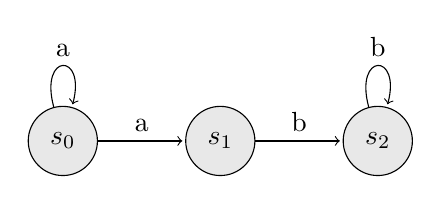
\begin{tikzpicture}[shorten >=1pt,node distance=2cm,on grid,auto] 
  \tikzstyle{every state}=[fill={rgb:black, 1;white,10}]

  \node[state] (s_0)                {$s_0$};
  \node[state] (s_1) [right of=s_0] {$s_1$};
  \node[state] (s_2) [right of=s_1] {$s_2$};

  \path[->]
  (s_0) edge [loop above] node {a} (   )
        edge              node {a} (s_1)
  (s_1) edge              node {b} (s_2)
  (s_2) edge [loop above] node {b} (   );
\end{tikzpicture}
\hspace{30pt}\rotatebox[origin=c]{0}{\scalebox{2.4}[3.6]{$\Rightarrow$}}\hspace{30pt}
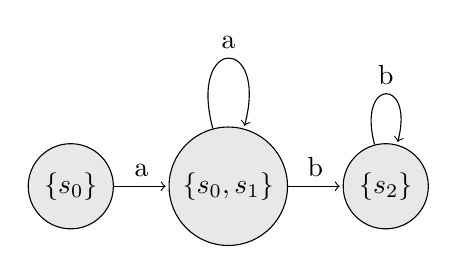
\begin{tikzpicture}[shorten >=1pt,node distance=2cm,on grid,auto] 
  \tikzstyle{every state}=[fill={rgb:black, 1;white,10}]

  \node[state] (s_0)                {$\{s_0\}$};
  \node[state] (s_1) [right of=s_0] {$\{s_0, s_1\}$};
  \node[state] (s_2) [right of=s_1] {$\{s_2\}$};


  \path[->]
  (s_0) edge              node {a} (s_1)
  (s_1) edge [loop above] node {a} ()
  (s_1) edge              node {b} (s_2)
  (s_2) edge [loop above] node {b} (   );
\end{tikzpicture}
\caption*{Nondeterministic $\Rightarrow$ deterministic LTS (ignoring states with
  no transitions)}
\end{figure}
in text the deterministic LTS $$(L', S', R') = (\{a, b\}, \powerset{S}, \{(\{s_0,
a, \{s_0, s_1\}), (\{s_0, s_1\}, a, \{s_0, s_1\}), (\{s_0\}, b, \{s_2\}),
(\{s_2\}, b, \{s_2\})\})$$

\item \textbf{(5)} Design an LTS with 11 states that describes the payment of at
  least 10 with units of 1, 2, 5 and 10. (no change).
  \\
  Let $a \oplus b \text{ denote } min\{a+b, 10\}$ or 
  \begin{equation*}
    \begin{split}
      L & = \{1, 2, 5, 10\}\\
      S & = \{0, 1, 2, 3, 4, 5, 6, 7, 8, 9, 10\}\\
      R & = \{\{n, 1, n \oplus 1\} \cup\{n, 2, n \oplus 2\} \cup \{n, 5, n \oplus 5\} \cup \{n, 10, n \oplus 10\} \mid n \in S\}
    \end{split}
  \end{equation*}

  \item \textbf{(6)} Show that in any given LTS, if $s'',\bm{v} \vdash^*_R s',
    \lambda$ and $s', \bm{u} \vdash^*_R s, \lambda$, then $s'', \bm{uv}
    \vdash^*_R s, \lambda$.
    \\
 $s'',\bm{v} \vdash^*_R s',\lambda$ means that our LTS contains the steps $s'
 \xrightarrow{v_0} \cdot \xrightarrow{v_1}...\xrightarrow{v_n}s''$ where $v_0,
 v_1,...,v_n$ are the symbols of $\bm{v}$. Similarly we have$s
 \xrightarrow{u_0} \cdot \xrightarrow{u_1}...\xrightarrow{u_n}s'$. We can
 concatenate these paths to form $s
 \xrightarrow{u_0} \cdot \xrightarrow{u_1}...\xrightarrow{u_n}s'
 \xrightarrow{v_0} \cdot \xrightarrow{v_1}...\xrightarrow{v_n}s''$ which means $s'', \bm{uv}
    \vdash^*_R s, \lambda$

  \item \textbf{(8)} Prove:\\(1) For any state $x \in S$ and word $\bm{w} \in
    L^*$, there exists a unique state $Y_{x,\bm{w}} \in \powerset{S}$ such that
    $Y_{x,\bm{w}}, \bm{w} \vdash^*_{R_\mathcal{P}} \{x\}, \lambda$.\\
    We prove (1) by induction on $\bm{w}$.\\
    Step 0:\[\bm{w} = \lambda \Rightarrow Y_{x, \bm{w}} = \{x\}\]
    $\{x\}$ is a unique set so (1) holds for the empty word.\\
    Induction step: Assume $Y_{x, \bm{w}}$ is a unique state, we look at $Y_{x,
      \bm{w}l}$ for some arbitrary label $l$. $Y_{x,\bm{w}l} = r(Y_{x,\bm{w}},
    l)$ and since $r$ is a function, this is a unique set.
  \end{itemize}
  \section*{main.pdf 5.6}
  
  \begin{itemize}[label=]
    \item \textbf{(2)} Let $(M, 1, \ast)$ be a finite monoid and
      $\varphi:\Sigma^{*} \rightarrow M$ a morhpishm from $(\Sigma^{*}, \lambda
      \cdot)$ to $(M, 1, \ast)$. Show that the image of a word is given by the
      images of its letters.\\\\
      We want to show $\varphi(l_1...l_n) =
      \varphi(l_1)\ast...\ast\varphi(l_n)$.
      \begin{equation*}
        \begin{split}
          \varphi(l_1...l_n) & = \varphi(l_1 \cdot ... \cdot l_n) \text{ a word is the concatenation of its letters}\\
          & = \varphi(l_1) \ast ... \ast \varphi(l_n) \text{ by the associativity of concatenation, and the morhpishm condition}
        \end{split}
      \end{equation*}
      \\\\
    Show that for every $F \subseteq M$, $L = \{\bm{w} \in \Sigma^{*} \mid
      \varphi(\bm{w}) \in F\}$ is regular.\\
    We construct a finite state machine $M_L = (\Sigma, M, q_0 R, A)$ (using A
    for the set of Accepting states) with:
    \begin{equation*}
      \begin{split}
        q_0 & = 1 \\
        A & = F \\
        R & = \{m \xrightarrow{l} m' \mid m, m' \in M, m \ast \varphi(l) = m'\}
      \end{split}
    \end{equation*}\\
    Accepting paths in this machine look like $1 \xrightarrow{l_1} 1 \ast
    \varphi(l_1) ... \xrightarrow{l_n} 1 \ast \varphi(l_1) \ast ... \ast
    \varphi(l_n) \in F$. By the morphism condition $1 \ast \varphi(l_1) \ast ... \ast \varphi(l_n) =
    \varphi(\lambda \cdot l_1...l_n) = \varphi(\bm{w})$ so this machine accepts
    $L$.
    \\\\
   Show that $L' = \{a^{\lvert \bm{w} \rvert}\mid \bm{w} \in L\}$ is a regular
   language.\\
   We can reuse the structure of $M_L$ to define a new FSM $M_{L'} = (\Sigma, M,
   q_0 R', F)$ with $R' = \{m \xrightarrow{a} m' \mid m \rightarrow{l} m' \in
   R\}$. This new machine has the same structure as $M_L$, but every label is
   $a$. It accepts $L'$.
  \item \textbf{(3)} Let $L$ be a language over $\Sigma$. For $\bm{v}, \bm{w}
    \in \Sigma^{*}$ define $\bm{v} \sim_L \bm{w} := \bm{vu} \in L \iff \bm{wu} \in
    L \text{ for all } \bm{u} \in \Sigma^{*}$.\\
    Show that $\sim_L$ is an equivalence relation:\\
    \begin{itemize}
      \item reflexive: $\bm{vu} = \bm{vu}$, so $\bm{v} \sim_L \bm{v}$
      \item symmetric: $\iff$ is symmetric, so $\sim_L$ is also
      \item transitive: let $\bm{x} \sim_L \bm{y}, \bm{y} \sim_L \bm{z}$. Then
        $\bm{xu} \in L \iff \bm{yu} \in L$ and $\bm{yu} \in L \iff \bm{zu} \in
        L$ so $\bm{xu} \in L \iff \bm{zu} \in L$
    \end{itemize}
   Show that all equivalence classes $[a^n], n \geq 0$ in $L = \{a^nb^n \mid n \geq
   0\}$ are different.\\
   $a^n\bm{u} \in L \iff \bm{u} = b^n$. Clearly $b^n \not = b^m$ for $n\not = m$
   so $[a^n]$ is different for each $n$.\\\\
   Show that all equivalence classes $[ba^n]$ are the same.\\
   There is no $\bm{u}$ s.t $ba^n\bm{u} \in L$ so $[ba^n]$ is the class of words
   that cannot be extended to be in $L$ for all $n$.
   \\\\
   Consider the LTS $(\Sigma, \Sigma^{*} / \sim_L, R_L)$ with $R_L = \{([\bm{w}],
   l, [\bm{w}l])\}$ Show that $R_L$ is well defined.\\
   We want to show that $\bm{v} \sim_L \bm{w} \implies (R_L([\bm{v}], l,
   [\bm{v}l]) \iff R_L([\bm{w}], l, [\bm{w}l]))$.\\
   $\bm{v} \sim_L \bm{w}$ means $\bm{vu} \in L \iff \bm{wu} \in L$ for all $\bm{u}
   \in \Sigma^{*}$. Consider $V = \{\bm{v} \in \Sigma^{*} \mid \bm{v} =
   l\bm{x}, \bm{x} \in \Sigma^{*}\} \subseteq \Sigma^{*}$ the subset of words
   starting with $l$. Since it is a subset, the equivalence implies $\bm{vu} \in
   L \iff \bm{wu} \in L$ for all $u \in V$, which means $\bm{v}l\bm{u} \in
   L \iff \bm{w}l\bm{v} \in L$ for all $u \in \Sigma^*$ -- the same as $\bm{v}l
   \sim_L \bm{w}l$. Hence $[\bm{v}] \sim_L \bm{w} \iff [\bm{v}l] \sim_L
   [\bm{w}l]$ and $R_L$ is well defined.\\\\
   Show that the LTS is deterministic.\\
   $R_L$ is injective and well defined, so it is a function. An LTS where the
   transition relation is a function is deterministic.
   \\\\
   Assume $L$ is accepted by some FSM $(\Sigma, Q, q_0, \Upsilon, F)$.\\
   Show that for any $q \in Q$ and words $\bm{v}, \bm{w} \in \Sigma^{*}$, if $q$
   is reachable from $q_0$ with both $\bm{v}$ and $\bm{w}$, then $\bm{v} \sim_L
   \bm{w}$.\\
   $q$ reachable from $q_0$ by $\bm{v}$ and $\bm{w}$ means there exists a path
   $q_0 \xrightarrow{l_0}...\xrightarrow{l_n} q$ such that $l_0 \cdot ... \cdot
   l_n = \bm{v}$ and one where $l_0 \cdot ... \cdot
   l_n = \bm{w}$. Consider $\bm{u}$ such that $\bm{u} = l_0 \cdot ... \cdot l_n$ and
   the path $q \xrightarrow{l_0}...\xrightarrow{l_n} q'$ is in the FSM (note
   that $\bm{u}$ could be the empty word, in which case $q = q'$). We can
   concatenate the paths to $q$ with the path described by $\bm{u}$. Then both
   $\bm{vu}$ and $\bm{wu}$ are in $L$ iff $q \in F$, so $\bm{v} \sim_L \bm{w}$.
   \\\\
   Show that $\Sigma^{*}/\sim_L$ is finite.\\
   Consider the function $\mu: [\bm{w}] \mapsto q \text{ reached by } \bm{w}
   \text{ from } q_0$. Our previous results shows that if two words both reach
   $q$, then they are in the same equivalence class, so $\mu$ is injective. We may
   assume every state is reachable by \textit{some} word without affecting the
   language accepted by our FSM, so $\mu$ is also surjective. Hence $\mu$ is a
   bijection $\Sigma^{*} / \sim_L \rightarrow Q$ and since $Q$ is finite, so is
   $\Sigma^{*} / \sim_L$.
   \\\\
   Prove that the language $L' = \{a^nb^n \mid n \geq 0\}$ is irregular. (Not
   accepted by an FSM).\\
   We have seen that an FSM $(\Sigma, Q, q_0, \Upsilon, F)$ which accepts $L$
   has $\lvert Q \rvert = \lvert \Sigma^{*}/\sim_L \rvert$. We have also seen
   that $[a^n]$ is distinct for each $n$. Hence $\lvert \Sigma^{*}/ \sim_{L'}
   \rvert$ is not finite, and there can be no FSM accepting $L'$. 
 \end{itemize}
 \section*{Book 3.1}
 \begin{itemize}[label=]
 \item \textbf{(2)} Which of the following are accepted?\\
   \textit{aaabab} and \textit{bbbabab} are accepted.
 \item \textbf{(3)} Write an expression for the language accepted by the
   automaton.\\
   $\{a^nb\mid n \geq 0 \} \cup \{(ba)^nb \mid n \geq 0\} = \{(a \vert ba)^nb
     \mid n \geq 0\}$
 \item \textbf{(6)} Write an expression for the language accepted by the
   automaton.\\
   $\{(a^n(a \vert b) ab)^ma^k(a \vert b)a \mid n, m, k \geq 0\}$
 \item \textbf{(15)} Find a deterministic automaton accepting the same language
   as the given automaton.\\
   \begin{figure}[H]
     \centering
     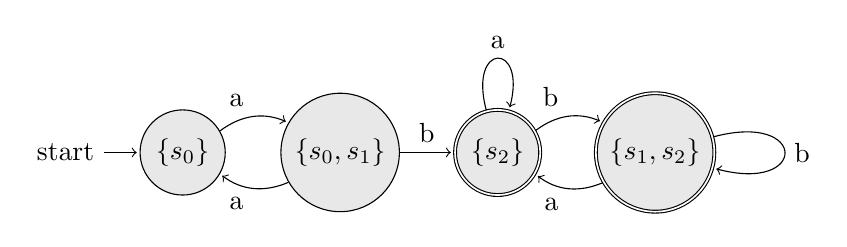
\begin{tikzpicture}[shorten >=1pt,node distance=2cm,on grid,auto]
       \tikzstyle{every state}=[fill={rgb:black, 1;white,10}]

       \node[state, initial] (s_0)                {$\{s_0\}$};
       \node[state]          (s_1) [right of=s_0] {$\{s_0, s_1\}$};
       \node[state,accepting](s_2) [right of=s_1] {$\{s_2\}$};
       \node[state,accepting](s_3) [right of=s_2] {$\{s_1, s_2\}$};

       \path[->]
       (s_0) edge [bend left] node {a} (s_1)
       (s_1) edge [bend left] node {a} (s_0)
             edge node {b} (s_2)
       (s_2) edge [loop above] node {a} ()
             edge [bend left] node {b} (s_3)
       (s_3) edge [loop right] node {b} ()
             edge [bend left]  node {a} (s_2);
     \end{tikzpicture}
     \caption{Deterministic automaton for (15)}
  \end{figure}
 \item \textbf{(18)} Find a deterministic automaton accepting the same language
   as the given automaton.\\
   \begin{figure}[H]
     \centering
     \begin{tikzpicture}[shorten >=1pt,node distance=2cm,on grid,auto]
       \tikzstyle{every state}=[fill={rgb:black, 1;white,10}]

       \node[state, initial] (s_0)                {$\{s_0\}$};
       \node[state]          (s_2) [above right of=s_1] {$\{s_1, s_2\}$};
       \node[state,accepting](s_3) [below right of=s_1] {$\{s_1, s_3\}$};
       \node[state]          (s_1) [below right of=s_2] {$\{s_1\}$};
       \node[state,accepting](s_4) [right of=s_1] {$\{s_2, s_3\}$};
       \node[state,accepting](s_5) [right of=s_4] {$\{s_3\}$};

       \path[->]
       (s_0) edge node {a} (s_2)
       (s_1) edge node {b} (s_3)
       (s_2) edge node {a} (s_1)
             edge node {b} (s_3)
       (s_3) edge [bend right] node {a} (s_4)
             edge [loop below] node {b} ()
       (s_4) edge [bend right] node {a} (s_2)
             edge [bend left] node {b} (s_5)      
       (s_5) edge [loop right] node {b} ()
             edge [bend left] node {a} (s_4);
     \end{tikzpicture}
     \caption{Deterministic automaton for (18)}
  \end{figure}
 \end{itemize}
 \section*{Book 3.2}
 \begin{itemize}[label=]
 \item \textbf{(2) a)} Given finite automata for $L_1$ and $L_2$, construct one
   that accepts $L_1 \cup L_2$. Note that the complete automata have been left
   out for the sake of my sanity.
   \begin{figure}[H]
     \centering
     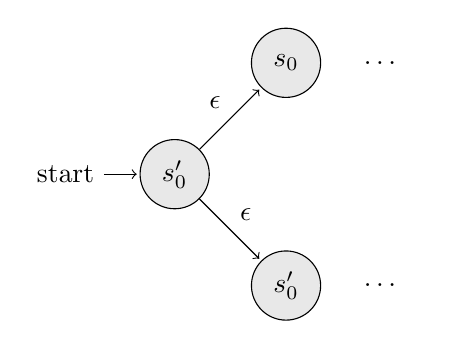
\begin{tikzpicture}[shorten >=1pt,node distance=2cm,on grid,auto]
       \tikzstyle{every state}=[fill={rgb:black, 1;white,10}]

       \node[state, initial] (s_0) {$s_0'$};
       \node[state] (s_1) [above right of=s_0] {$s_0$};
       \node[state] (s_2) [below right of=s_0]{$s_0'$};
       \coordinate[right =of s_1] (d_1);
       \coordinate[right =of s_2] (d_2);

       \path[->]
       (s_0) edge node {$\epsilon$} (s_1)
             edge node {$\epsilon$} (s_2);

       \path (s_1) -- node[auto=false] {\ldots} (d_1);
       \path (s_2) -- node[auto=false] {\ldots} (d_2);
     \end{tikzpicture}
     \caption{$L_1 \cup L_2$}
  \end{figure}
  \item \textbf{(b)} construct an automata for $L_1 \cdot L_2$
   \begin{figure}[H]
     \centering
     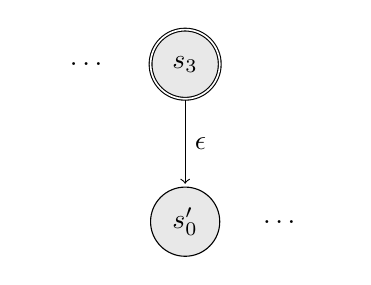
\begin{tikzpicture}[shorten >=1pt,node distance=2cm,on grid,auto]
       \tikzstyle{every state}=[fill={rgb:black, 1;white,10}]

       \node[state, accepting] (s_3) {$s_3$};
       \node[state] (s_0) [below =of s_3] {$s_0'$};
       \coordinate[left =of s_3] (d_3);
       \coordinate[right =of s_0] (d_0);

       \path[->]
       (s_3) edge node {$\epsilon$} (s_0);

       \path (s_3) -- node[auto=false] {\ldots} (d_3);
       \path (s_0) -- node[auto=false] {\ldots} (d_0);
     \end{tikzpicture}
     \caption{$L_1 \cdot L_2$}
  \end{figure}
  \item \textbf{(c)} construct automata for $L_1^*$ and $L_2^*$
   \begin{figure}[H]
     \centering
     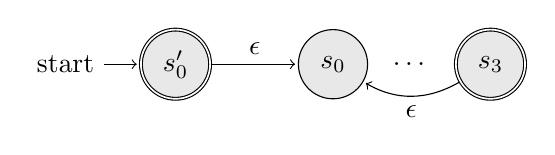
\begin{tikzpicture}[shorten >=1pt,node distance=2cm,on grid,auto]
       \tikzstyle{every state}=[fill={rgb:black, 1;white,10}]

       \node[state, initial, accepting] (s_0) {$s_0'$};
       \node[state] (s_1) [right =of s_0]{$s_0$};
       \node[state, accepting] (s_2) [right =of s_1]{$s_3$};

       \path[->]
       (s_0) edge node {$\epsilon$} (s_1)
       (s_2) edge [bend left] node {$\epsilon$} (s_1);

       \path (s_1) -- node[auto=false] {\ldots} (s_2);
     \end{tikzpicture}
     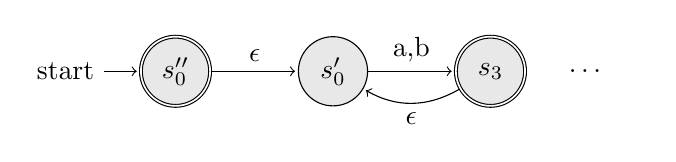
\begin{tikzpicture}[shorten >=1pt,node distance=2cm,on grid,auto]
       \tikzstyle{every state}=[fill={rgb:black, 1;white,10}]

       \node[state, initial, accepting] (s_0) {$s_0''$};
       \node[state] (s_1) [right =of s_0]{$s_0'$};
       \node[state, accepting] (s_2) [right =of s_1]{$s_3$};
       \coordinate[right =of s_2] (d_2);

       \path[->]
       (s_0) edge node {$\epsilon$} (s_1)
       (s_1) edge node {a,b} (s_2)
       (s_2) edge [bend left] node {$\epsilon$} (s_1);

       \path (s_2) -- node[auto=false] {\ldots} (d_2);
     \end{tikzpicture}
     \caption{Automata for $L_1^*$ (left) and $L_2^*$ (right)}
  \end{figure}
 \item \textbf{(5)} Use transition graphs to construct the regular language
   accepted by the automaton.\\
   We construct the following transition graph and determine that the accepted
   language is $\{b^nab^mab^ka \mid n,m,k \geq 0\}$.
   \begin{figure}[H]
     \centering
     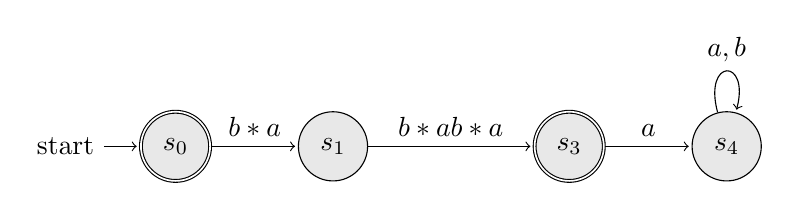
\begin{tikzpicture}[shorten >=1pt,node distance=2cm,on grid,auto]
       \tikzstyle{every state}=[fill={rgb:black, 1;white,10}]

       \node[state, initial, accepting] (s_0) {$s_0$};
       \node[state] (s_1) [right =of s_0]{$s_1$};
       \node[state, accepting] (s_2) [right = 3cm of s_1]{$s_3$};
       \node[state] (s_3) [right =of s_2]{$s_4$};

       \path[->]
       (s_0) edge node {$b*a$} (s_1)
       (s_1) edge node {$b*ab*a$} (s_2)
       (s_2) edge node {$a$} (s_3)
       (s_3) edge [loop above] node {$a,b$} ();

     \end{tikzpicture}
     \caption{The transition graph for (5)}
\end{figure}
\item \textbf{(7)} Use transition graphs to construct the regular language
  accepted by the automaton.\\
   \begin{figure}[H]
     \centering
     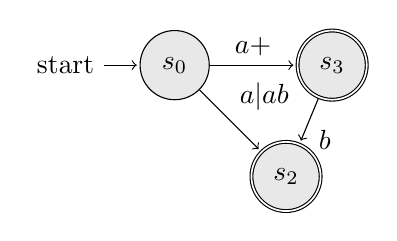
\begin{tikzpicture}[shorten >=1pt,node distance=2cm,on grid,auto]
       \tikzstyle{every state}=[fill={rgb:black, 1;white,10}]

       \node[state, initial] (s_0) {$s_0$};
       \node[state, accepting] (s_3) [right =of s_0]{$s_3$};
       \node[state, accepting] (s_2) [below right =of s_0]{$s_2$};

       \path[->]
       (s_0) edge node {$a+$} (s_3)
             edge node {$a \vert ab$} (s_2)
       (s_3) edge node {$b$} (s_2);

     \end{tikzpicture}
     \caption{The transition graph for (7)}
   \end{figure}
   We note that the accepted language is $a+ \vert a \vert ab \vert a+b$ (where
   $+$ denotes one or more occurences of the preceding letter) which simplifies
   to $a+ \vert a+b$
 \end{itemize}
\end{document}
